\documentclass[11pt]{article}
\usepackage{amsmath}
\usepackage{amssymb}
\usepackage{amsthm}
\usepackage{tikz}
\usepackage{geometry}
\geometry{margin=1in}

\DeclareMathOperator*{\argmax}{arg\,max}

\title{Deriving DT Loss with Simple Example}
\author{}
\date{}

\begin{document}
\maketitle

\section{Setup}
Let's derive DT loss with simple example:

We have a two frame video: $X_1, X_2$

Each frame has a noise level:
$K \sim \text{Uniform}(0, K)$ where 0 is no noise, $K$ is full.

So $X_1^{K_1}, X_2^{K_2}$ are the two frames with their noise levels $K_1, K_2$ respectively.

\section{Objective}
Let us define our goal:
\begin{align}
\argmax_\theta \mathbb{E}_{X_1^0, X_2^0 \sim p_{\text{data}}} \left[ \ln(p_\theta(X_1^0, X_2^0)) \right]
\end{align}

We derive a surrogate objective via the ELBO:
\begin{align}
\mathbb{E}_{X_1^0, X_2^0} \left[ \ln(p_\theta(X_1^0, X_2^0)) \right]
\end{align}

\begin{align}
= \mathbb{E}_{X_1^0, X_2^0} \left[ \ln \int p_\theta(X_1^0, X_2^0, X_1^{i:K}, X_2^{i:K}) dX_1^{i:K} dX_2^{i:K} \right]
\end{align}

Let's assume a Gaussian noising process:
\begin{align}
q(X_i^k | X_i^0) &\sim \alpha_K X_i^0 + \beta_K \epsilon, \quad \epsilon \sim \mathcal{N}(0, I) \\
&\sim \mathcal{N}(\alpha_K X_i^0, \beta_K I)
\end{align}

\begin{align}
&= \mathbb{E}_{X_1^0, X_2^0} \left[ \ln \int p(X_1^{0:K}, X_2^{0:K}) \cdot \frac{q(X_1^{1:K}, X_2^{1:K} | X_1^0, X_2^0)}{q(X_1^{1:K}, X_2^{1:K} | X_1^0, X_2^0)} dX_1^{1:K} dX_2^{1:K} \right] \\
&= \mathbb{E}_{X_1^0, X_2^0 \sim p_{\text{data}}} \left[ \ln \mathbb{E}_{X_1^{1:K}, X_2^{1:K} \sim q(\cdot | X_1^0, X_2^0)} \left[ \frac{p(X_1^{0:K}, X_2^{0:K})}{q(X_1^{1:K}, X_2^{1:K} | X_1^0, X_2^0)} \right] \right] \\
&\geq \mathbb{E}_{X_1^0, X_2^0 \sim p_{\text{data}}, X_1^{1:K}, X_2^{1:K} \sim q(\cdot | X_1^0, X_2^0)} \left[ \ln \left[ \frac{p(X_1^{0:K}, X_2^{0:K})}{q(X_1^{1:K}, X_2^{1:K} | X_1^0, X_2^0)} \right] \right]
\end{align}

\begin{align}
p(X_1^{0:K}, X_2^{0:K}) = p(X_1^K, X_2^K) \prod_{i \in \tau} p(T_{i-1} | T_i), \quad \tau \sim \text{Traj}(2,K)
\end{align}

where $T_i$ is the ith state in a trajectory, but always: $T_0 = (X_1^0, X_2^0)$, $T_K = (X_1^K, X_2^K)$.

Traj$(2, K)$ is the set of all trajectories on a 2-dimensional cube with $K$ delimiters. From 0 vertex to the opposite vertex. Note that we can construct the joint distribution in any order according to the denoising trajectories we allow, and we can assign any probability distribution over these trajectories. This flexibility allows us to model different generative processes by choosing different trajectory distributions. In the general case beyond the 2-frame example, we would replace 2 with $n$ to get Traj$(n, K)$, representing trajectories on an $n$-dimensional cube.

\begin{align}
= \mathbb{E}_{X_1^{0:K}, X_2^{0:K}} \left[ \ln p(X_1^K, X_2^K) + \sum_{T_i \in \text{Traj}(2,K)} \ln \left( \frac{p(T_{i-1} | T_i)}{q(T_i | T_{i-1})} \right) \right]
\end{align}

\begin{align}
= \mathbb{E}_{X_1^{0:K}, X_2^{0:K}} \left[ \ln p(X_1^K, X_2^K) \right] + \sum_{T_i \in \text{Traj}(2,K)} \mathbb{E}_{T_{i-1}, T_i} \left[ \ln \left( \frac{p(T_{i-1} | T_i) \cdot q(T_{i-1})}{q(T_{i-1} | T_i) \cdot q(T_i)} \right) \right]
\end{align}

We take all constants w.r.t $p$ out:
\begin{align}
\mathbb{E}_{X_1^K, X_2^K} \left[ \ln p(X_1^K, X_2^K) \right] + \sum_{T_i \in \text{Traj}(2,K)} \mathbb{E}_{T_{i-1}, T_i} \left[ \ln \left( \frac{p(T_{i-1} | T_i)}{q(T_{i-1} | T_i)} \right) \right]
\end{align}

\begin{align}
= \mathbb{E}_{X_1^K, X_2^K} \left[ \ln p(X_1^K, X_2^K) \right] - \sum_{T_i \in \text{Traj}(2,K)} D_{KL}(q(T_{i-1} | T_i) || p(T_{i-1} | T_i))
\end{align}

Note that $q(X_1^K, X_2^K) = p(X_1^K, X_2^K) = \mathcal{N}(0, I)$, and our model parameters typically do not change $p(X_1^K, X_2^K)$, so we can discard the first term. This gives us a simple sum of KL divergences over trajectories sampled from our trajectory distribution:
\begin{align}
\mathcal{L} = \sum_{\tau \sim \text{Traj}(2,K)} \sum_{i \in \tau} D_{KL}(q(T_{i-1} | T_i) || p(T_{i-1} | T_i))
\end{align}

The probabilities assigned to each trajectory should correspond to the importance of each trajectory when sampling from the model. Recall that each trajectory can be decomposed as a sequence of transitions from $T_i$ to $T_{i-1}$ (denoising steps). Our loss can also be written as an expectation over trajectory states:
\begin{align}
\mathcal{L} = \mathbb{E}_{\tau \sim \text{Traj}(2,K)} \left[ \mathbb{E}_{T_i \in \tau} \left[ D_{KL}(q(T_{i-1} | T_i) || p(T_{i-1} | T_i)) \right] \right]
\end{align}

Or equivalently as a weighted sum over all possible trajectories:
\begin{align}
= \sum_{\tau \in \text{Traj}(2,K)} p(\tau) \sum_{T_i \in \tau} D_{KL}(q(T_{i-1} | T_i) || p(T_{i-1} | T_i))
\end{align}

If we instead write this as probaability distributions over atomic transitions marginalized over the distribution of trajectories, we get:

\begin{align}
= \sum_{T_i \rightarrow T_{i-1} \in \text{Traj}(2,K)} P(T_i \rightarrow T_{i-1}) D_{KL}(q(T_{i-1} | T_i) || p(T_{i-1} | T_i))
\end{align}

\section{Generalizing to the n-frame case}

To generalize to the n-frame case, we jsut chnage 2 to n.

\begin{align}
\sum_{T_i \in \text{Traj}(n,K)} P(T_i \rightarrow T_{i-1}) D_{KL}(q(T_{i-1} | T_i) || p(T_{i-1} | T_i))
\end{align}

In DF paper it applies equal probability to each transition:
\begin{align}
P(T_{i-1} \rightarrow T_i) = P(T_{j-1} \rightarrow T_j) 
\end{align}

but this should not be the case if we never double back and assign equal probability to each trajectory (you expect transitions of states near the diagonal to be weighted more by the binomial Thm).

Practically, this should not matter too much but good to keep in mind that our prior over Trajectories is not uniform (but over transitions is).

% If we asssume equal probability for each trajectory in DF, our weights should be proportional to:

% \begin{align}
% \begin{pmatrix}
% K_1 + \cdots + K_n - 1 \\
% K_1, K_2, \cdots, K_i - 1, \cdots, K_n
% \end{pmatrix} + \begin{pmatrix}
% (K - K_1) + \cdots + (K - K_n) \\
% K - K_1, \cdots, K - K_n
% \end{pmatrix}
% \end{align}

% \begin{align}
% = \begin{pmatrix}
% n \cdot K \\
% K, K, \cdots, K
% \end{pmatrix}_{n \text{ times}}
% \end{align}

Also, in an architecture like the Transformer, our state transitions decrease the noise level of each frame by 1, so the space of trajectories looks more like a diagonal pattern, but this proof still holds as we did not make any assumptions about the transitions allowed as long as they they are steadily denoising the frames.


\begin{center}
    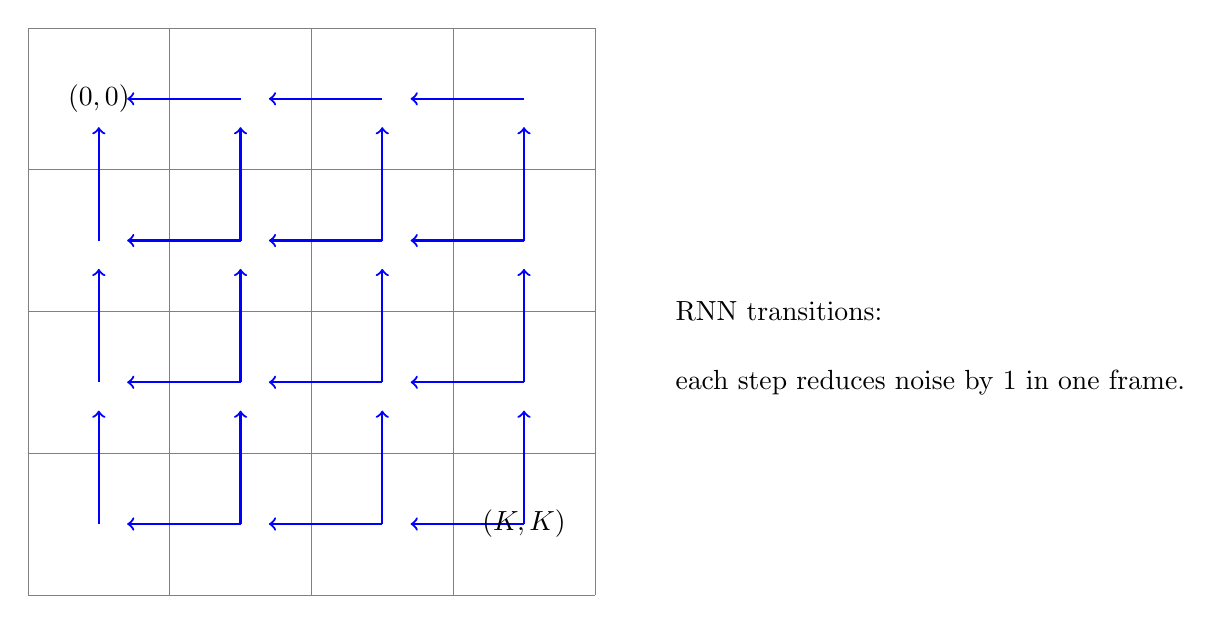
\begin{tikzpicture}[scale=1.8]
    \draw[step=1cm,gray,very thin] (0,0) grid (4,4);
    % Interior points with up and left arrows (no diagonals)
    \foreach \x in {1,2,3} {
      \foreach \y in {0,1,2} {
        \draw[->,thick,blue] (\x+0.5,\y+0.5) -- (\x-0.3,\y+0.5);
        \draw[->,thick,blue] (\x+0.5,\y+0.5) -- (\x+0.5,\y+1.3);
      }
    }
    % Left edge (only up arrows)
    \foreach \y in {0,1,2} {
      \draw[->,thick,blue] (0.5,\y+0.5) -- (0.5,\y+1.3);
    }
    % Top row (only left arrows)
    \foreach \x in {1,2,3} {
      \draw[->,thick,blue] (\x+0.5,3.5) -- (\x-0.3,3.5);
    }
    % Corner labels
    \node at (0.5,3.5) {$(0,0)$};
    \node at (3.5,0.5) {$(K,K)$};
    \node[anchor=west] at (4.5,2) {RNN transitions:};
    \node[anchor=west] at (4.5,1.5) {each step reduces noise by 1 in one frame.};
    \end{tikzpicture}
    \end{center}
    

\begin{center}
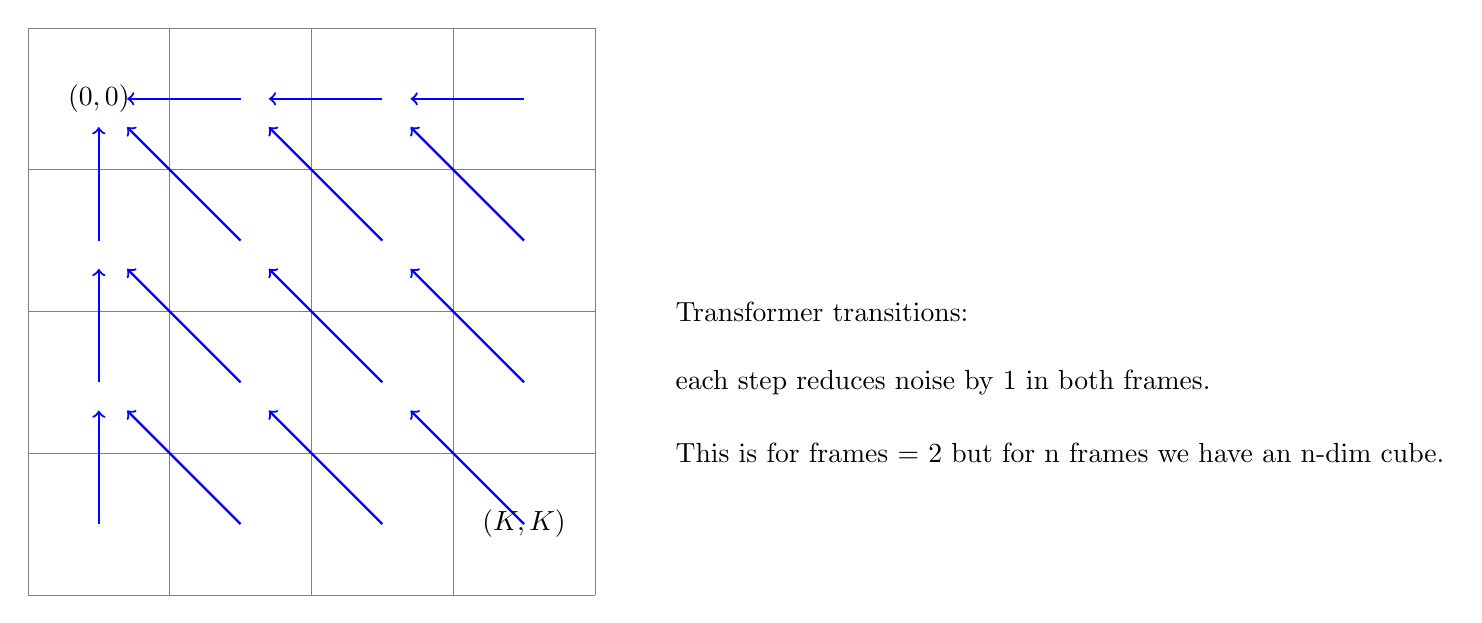
\begin{tikzpicture}[scale=1.8]
\draw[step=1cm,gray,very thin] (0,0) grid (4,4);
% Interior points with diagonal arrows (up-left)
\foreach \x in {1,2,3} {
  \foreach \y in {0,1,2} {
    \draw[->,thick,blue] (\x+0.5,\y+0.5) -- (\x-0.3,\y+1.3);
  }
}
% Left edge (only up arrows)
\foreach \y in {0,1,2} {
  \draw[->,thick,blue] (0.5,\y+0.5) -- (0.5,\y+1.3);
}
% Top row (only left arrows)
\foreach \x in {1,2,3} {
  \draw[->,thick,blue] (\x+0.5,3.5) -- (\x-0.3,3.5);
}
% Corner labels
\node at (0.5,3.5) {$(0,0)$};
\node at (3.5,0.5) {$(K,K)$};
\node[anchor=west] at (4.5,2) {Transformer transitions:};
\node[anchor=west] at (4.5,1.5) {each step reduces noise by 1 in both frames.};
\node[anchor=west] at (4.5,1) {This is for frames = 2 but for n frames we have an n-dim cube.};
\end{tikzpicture}
\end{center}


TF is encapsulated in this framework too.

TF weights should be a constant traversing the edge of the cube from frame 1 $\rightarrow$ frame 2 $\rightarrow$ ... denoising which is:

\begin{align}
\mathbb{I}\left( \left\{ X_1^0, X_2^0, \ldots, X_i^{K_i}, X_{i+1}^K, \ldots, X_n^K \right\} \rightarrow \left\{ X_1^0, X_2^0, \ldots, X_i^{K_i-1}, X_{i+1}^K, \ldots, X_n^{1K} \right\} \right)
\end{align}

i.e. pick any frame $i$, every frame to the left should be clean, every frame to the right should be full noise, and the transition should be denoising the $i$th frame by 1 noise level.


\section{Deriving the Self-Forcing Objective and Training Algorithm}

Let's derive the self-forcing objective and training algorithm from the following:

Instead of $\argmax_\theta \mathbb{E}_{X \sim p_{\text{data}}} \left[ \ln(p_\theta(X)) \right]$,

we swap $p_{\text{data}}$ and $p_\theta$ to get:
\begin{align}
\argmax_\theta \mathbb{E}_{X_1^0, X_2^0 \sim p_\theta} \left[ \ln(p_{\text{data}}(X_1^0, X_2^0)) \right]
\end{align}

\begin{align}
= \argmax_\theta \mathbb{E}_{X_1^0, X_2^0 \sim p_\theta} \left[ \ln \int p_{\text{data}}(X_1^{0:K}, X_2^{0:K}) \cdot \frac{p_\theta(X_1^{1:K}, X_2^{1:K} | X_1^0, X_2^0)}{p_\theta(X_1^{1:K}, X_2^{1:K} | X_1^0, X_2^0)} dX_1^{1:K} dX_2^{1:K} \right]
\end{align}

\begin{align}
= \argmax_\theta \mathbb{E}_{X_1^0, X_2^0 \sim p_\theta, } \left[ \ln \mathbb{E}_{X_1^{1:K}, X_2^{1:K} \sim p_\theta(\cdot | X_1^0, X_2^0)} \left[ \frac{p_{\text{data}}(X_1^{0:K}, X_2^{0:K})}{p_\theta(X_1^{1:K}, X_2^{1:K} | X_1^0, X_2^0)} \right] \right]
\end{align}

\begin{align}
\geq \argmax_\theta \mathbb{E}_{X_1^{0:K}, X_2^{0:K} \sim p_\theta} \left[ \ln \left( \frac{p_{\text{data}}(X_1^{0:K}, X_2^{0:K})}{p_\theta(X_1^{1:K}, X_2^{1:K} | X_1^0, X_2^0)} \right) \right]
\end{align}

\end{document}